\documentclass[12pt,a4paper,oneside]{report}
% CREATED BY DAVID FRISK, 2016

% BASIC SETTINGS
\usepackage{moreverb}								% List settings
\usepackage{textcomp}								% Fonts, symbols etc.
\usepackage{lmodern}								% Latin modern font
\usepackage{helvet}									% Enables font switching
\usepackage[T1]{fontenc}							% Output settings
\usepackage[english]{babel}							% Language settings
\usepackage[utf8]{inputenc}							% Input settings
\usepackage{amsmath}								% Mathematical expressions (American mathematical society)
\usepackage{amssymb}								% Mathematical symbols (American mathematical society)
\usepackage{graphicx}								% Figures
\usepackage{subfig}									% Enables subfigures
\numberwithin{equation}{chapter}					% Numbering order for equations
\numberwithin{figure}{chapter}						% Numbering order for figures
\numberwithin{table}{chapter}						% Numbering order for tables
\usepackage{minted}						    		% Enables source code listings
\usepackage{chemfig}								% Chemical structures
\usepackage[top=3cm, bottom=3cm,
			inner=3cm, outer=3cm]{geometry}			% Page margin lengths			
\usepackage{eso-pic}								% Create cover page background
\newcommand{\backgroundpic}[3]{
	\put(#1,#2){
	\parbox[b][\paperheight]{\paperwidth}{
	\centering
	\includegraphics[width=\paperwidth,height=\paperheight,keepaspectratio]{#3}}}}
\usepackage{float} 									% Enables object position enforcement using [H]
\usepackage{parskip}								% Enables vertical spaces correctly 
\usepackage{datetime} %date formatting tools


% OPTIONAL SETTINGS (DELETE OR COMMENT TO SUPRESS)

% Disable automatic indentation (equal to using \noindent)
\setlength{\parindent}{0cm}                         


% Caption settings (aligned left with bold name)
\usepackage[labelfont=bf, textfont=normal,
			justification=justified,
			singlelinecheck=false]{caption} 		

		  	
% Activate clickable links in table of contents  	
\usepackage{hyperref}								
\hypersetup{colorlinks, citecolor=black,
   		 	filecolor=black, linkcolor=black,
    		urlcolor=black}


% Define the number of section levels to be included in the t.o.c. and numbered	(3 is default)	
\setcounter{tocdepth}{5}							
\setcounter{secnumdepth}{5}	


% Chapter title settings
\usepackage{titlesec}		
\titleformat{\chapter}[display]
  {\Huge\bfseries\filcenter}
  {{\fontsize{50pt}{1em}\vspace{-4.2ex}\selectfont \textnormal{\thechapter}}}{1ex}{}[]


% Header and footer settings (Select TWOSIDE or ONESIDE layout below)
\usepackage{fancyhdr}								
\pagestyle{fancy}  
\renewcommand{\chaptermark}[1]{\markboth{\thechapter.\space#1}{}} 


% Select one-sided (1) or two-sided (2) page numbering
\def\layout{2}	% Choose 1 for one-sided or 2 for two-sided layout
% Conditional expression based on the layout choice
\ifnum\layout=2	% Two-sided
    \fancyhf{}			 						
	\fancyhead[LE,RO]{\nouppercase{ \leftmark}}
	\fancyfoot[LE,RO]{\thepage}
	\fancypagestyle{plain}{			% Redefine the plain page style
	\fancyhf{}
	\renewcommand{\headrulewidth}{0pt} 		
	\fancyfoot[LE,RO]{\thepage}}	
\else			% One-sided  	
  	\fancyhf{}					
	\fancyhead[C]{\nouppercase{ \leftmark}}
	\fancyfoot[C]{\thepage}
\fi


% Enable To-do notes
\usepackage[textsize=tiny]{todonotes}   % Include the option "disable" to hide all notes
\setlength{\marginparwidth}{2.5cm} 


% Supress warning from Texmaker about headheight
\setlength{\headheight}{15pt}		





\newcommand {\institutionfont}{\fontsize {22}{30}\scshape}
\newcommand {\divisionfont}{\fontsize {16}{20}\rmfamily}
\newcommand {\pretitlefont}{\fontsize {16}{16}\rmfamily}
\newcommand {\customtitlefont}{\fontsize {21}{28}\scshape}% {iwona}{bx}{n}}
\newcommand {\fixednamesfont}{\fontsize {14}{20}\mdseries}
\newcommand {\namesfont}{\fontsize {14}{20}\bfseries}
\newcommand {\footfont}{\fontsize {15}{18}\rmfamily}


\newcommand{\thesistitle}{A FPGA-based tensor accelerator for Machine Learning}
\newcommand{\thesisuniversitylogo}{images/logo/logoPoliTo_symbol_only} % choose your logo
\newcommand{\thesiscandidatename}{Francesco}
\newcommand{\thesiscandidatesurname}{Angione}
\newcommand{\thesissupervisoronetitle}{prof.}
\newcommand{\thesissupervisoronename}{Paolo}
\newcommand{\thesissupervisoronesurname}{Bernardi}
\newcommand{\thesissupervisortwotitle}{prof.}
\newcommand{\thesissupervisortwoname}{Pedro Petersen}
\newcommand{\thesissupervisortwosurname}{Moura Trancoso}
\newcommand{\thesisdate}{A.Y. 2019/2020}
\newcommand{\thesiscourse}{COURSE}
\newcommand{\thesisuniversity}{UNIVERSITY}
\newcommand{\thesislevel}{LEVEL} % master or bachelor
\newcommand{\thesiscandidatetext}{Candidate}
\newcommand{\thesissupervisortext}{Supervisors}



\begin{document}
\title{\vspace*{-5mm}\textbf{\thesistitle}\\Summary} % vspace is needed to shift upwards the title
\date{\thesisdate}
\author{\textbf{Candidate}:\\\thesiscandidatename~\thesiscandidatesurname\\
\textbf{Supervisors}:\\\thesissupervisoronetitle~\thesissupervisoronename~\thesissupervisoronesurname\\
\thesissupervisortwotitle~\thesissupervisortwoname~\thesissupervisortwosurname\\
}%\thesissupervisorthreetitle~\thesissupervisorthreename~\thesissupervisorthreesurname}

\maketitle


% CREATED BY DAVID FRISK, 2016
\chapter{Introduction}
Machine learning is one of the hot technologies today as it is being used to solve complex problems that would otherwise be very hard or costly to solve with traditional methods.\\The use of commodity hardware is not the most effective and efficient way to execute Machine Learning, so the goal is to satisfy the required demands for different Machine-Learning models but at lower cost and energy consumption in order to be deployed also on mobile devices.
As it is very well-known, hardware accelerators are capable, if designed correctly, of delivering a lot of improvements in terms of the latency but also in terms of energy efficiency. Thus, in order to obtain the best solution in every metric a hardware-software co-design is needed, requiring to the hardware designer a basic knowledge of machine learning algorithms.\\\\
The goal is to develop a hardware accelerator from scratch, which implements a tensor-based convolution. Exploiting a non Von Neumann architecture and reuse of weights reduces the CPU workload and boost the models' performance. The use of different arithmetic data type can drastically reduce the computations without reducing the final accuracy of the Neural Network. From a hardware perspective, the use of different arithmetic precision, such as the use of integer operations instead of floating-point operations, can lead to benefits in terms of area, energy consumption and latency.

%% CREATED BY DAVID FRISK, 2016
\chapter{Background}

\epigraph{ \textit{Can a machine think?}}{--- \textup{Alan Turing}, Computing Machinery and Intelligence}

\section{Overview}
In the past decade many companies have started to advertise the use of AI, even if they are using a subfield of the AI, in their products and software applications. Nevertheless, the recent growth,
the AI is not youth.\\ It takes one of its roots from a theoretical paper of \textit{Alan Turing} published by journal \textit{Mind} in the 1950 \cite{paper:36}.\\

The general definition of Artificial Intelligence (AI): \textit{intelligence demonstrated by machines, any device that perceives its environment and takes actions that maximize its chance of successfully achieving its goals}    \cite{book:1}.\\ In general, ''artificial intelligence'' is used when machines mimics the cognitive functions of the human mind, i.e. learning and problem solving.\\\\
According to the definition, AI is too vast to be studied and simulated \cite{book:1}. Therefore, it has been divided into subfields, characterized by different traits, such as knowledge representation, planning, learning, natural language processing, perception, motion and manipulation, social intelligence and general intelligence.\\\\

Artificial Intelligence can be seen as a general purpose technology. It does not exist a general task on which it excels neither how to characterize them.

\begin{figure}[H]
\centering
\captionsetup{justification=centering}
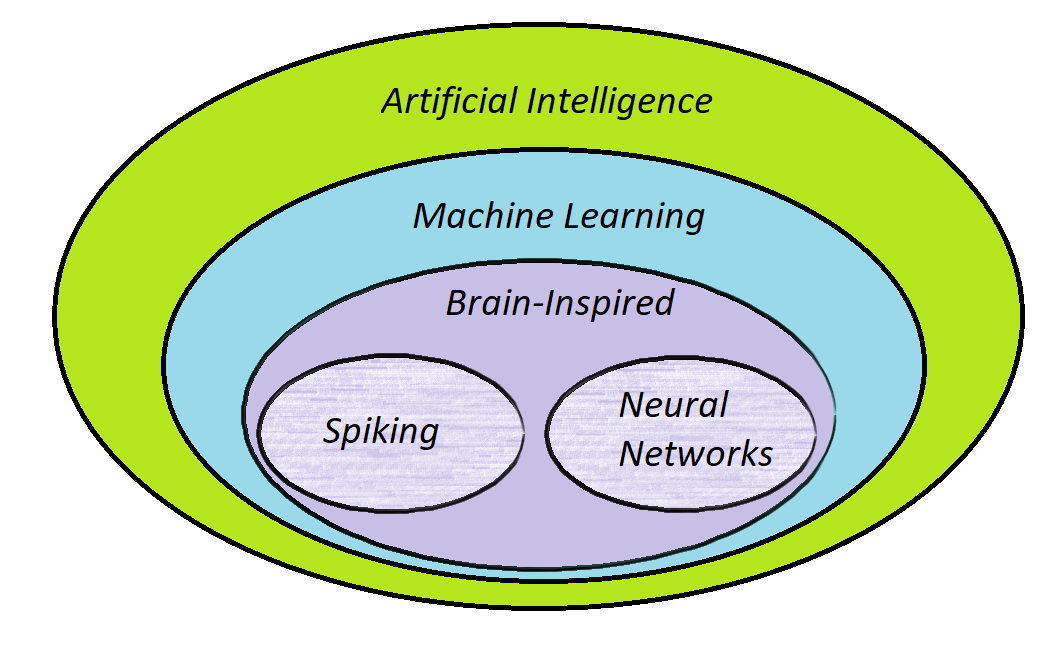
\includegraphics[scale=0.5]{./figure/ai_division.png}
\caption{Classification of AI with emphasis on Machine Learning and its subclassification}
\label{fig:aidiv}
\end{figure}

\section{Machine Learning}
A particular interesting subcategory of AI in Computer Science is the machine learning. It is the study of algorithms used to perform a specific task without explicit programming the machine, relying on patterns and inference, in order to make decisions.\\ This approach is used where it is tricky, or unfeasible, to develop a conventional algorithm for solving the task.\\

A peculiarity of machine learning model is that it is composed of two processes, training and inference.\\
The inference process is the process in which a conclusion is given at the end of the evaluation process, i.e. the input stimulus are applied to the model and the output is observed.\\
The training process has to be done before the model is put on the field, before the inference process, otherwise the latter can give wrong results. As the name suggests, in this process the model learns how to behave, adjusting the weight accordingly to the applied inputs and expected outputs. \\\\Besides this type of training and according to \cite{book:1}, other exists, characterized by approach, type of data and tasks:
\begin{itemize}
\item Supervised Learning, it builds a mathematical model of a set of data that contains both the inputs and the desired outputs.
\item Unsupervised Learning, it takes a set of data that contains only inputs and find structure in the data.
\item Semi-supervised Learning, it falls between unsupervised learning and supervised learning.
\item Reinforcement Learning, it concerns how software agents should take actions in order to maximize some notion.
\item Self Learning, It is a learning with no external rewards and no external teacher advices.
\item Feature Learning, also called representation learning algorithms, often attempts to transform data and preserve at the same time. It is used as a preprocessing step before any classification or predictions.
\item Sparse Dictionary Learning, it is a feature learning method where a training example is represented as a linear combination of basis functions, and is assumed to be a sparse matrix.
\item Anomaly Detection, also known as outlier detection,
identifies rare items, events or observations which are significantly different from the majority of data.
\item Association Rules, it is a rule-based method for discovering relationships between variables in large databases.
\end{itemize}

Machine learning space is also divided into other type of models such as decision tree, support vector machines, regression analysis, Bayesian networks and genetic algorithms.
As it can be seen in Figure \ref{fig:aidiv} Brain Inspired machine learning is also divided in subcategories.
\subsection{Brain Inspired}
It is based on algorithms which take its basic functionalities from our understanding of how the brain operates, trying to mimic the functionalities.
\begin{figure}[H]
\centering
\captionsetup{justification=centering}
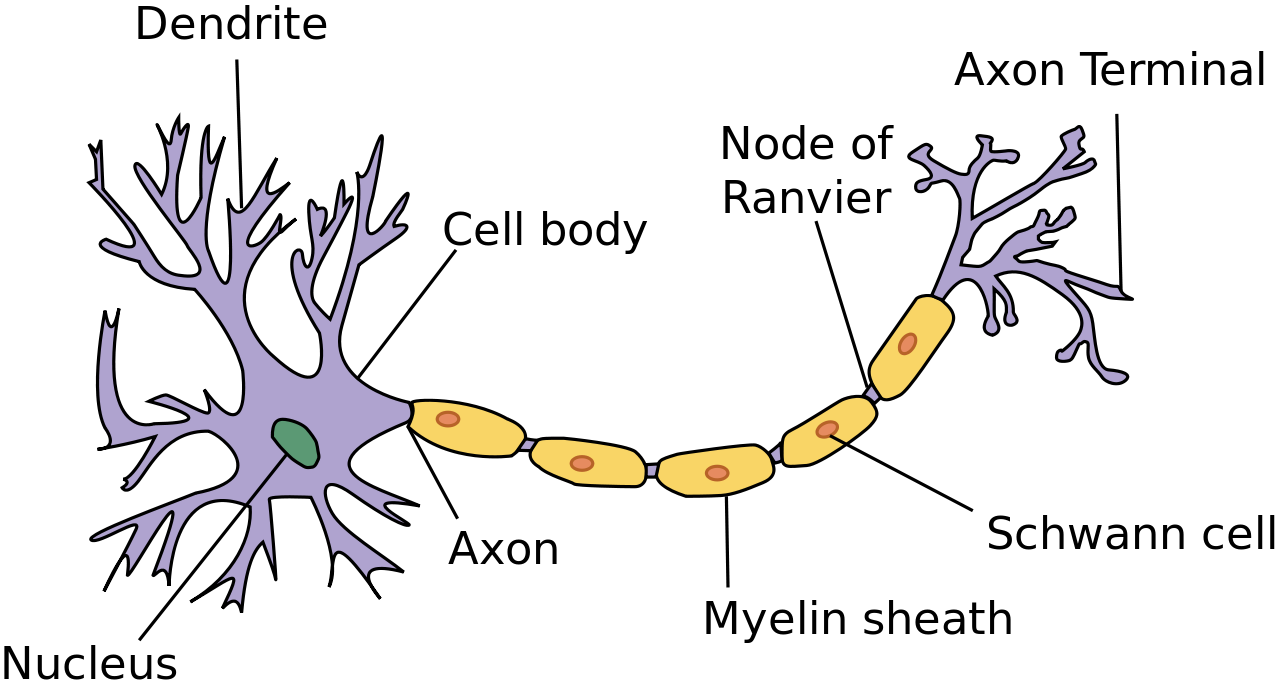
\includegraphics[scale=0.15]{./figure/human_neuron.png}\\

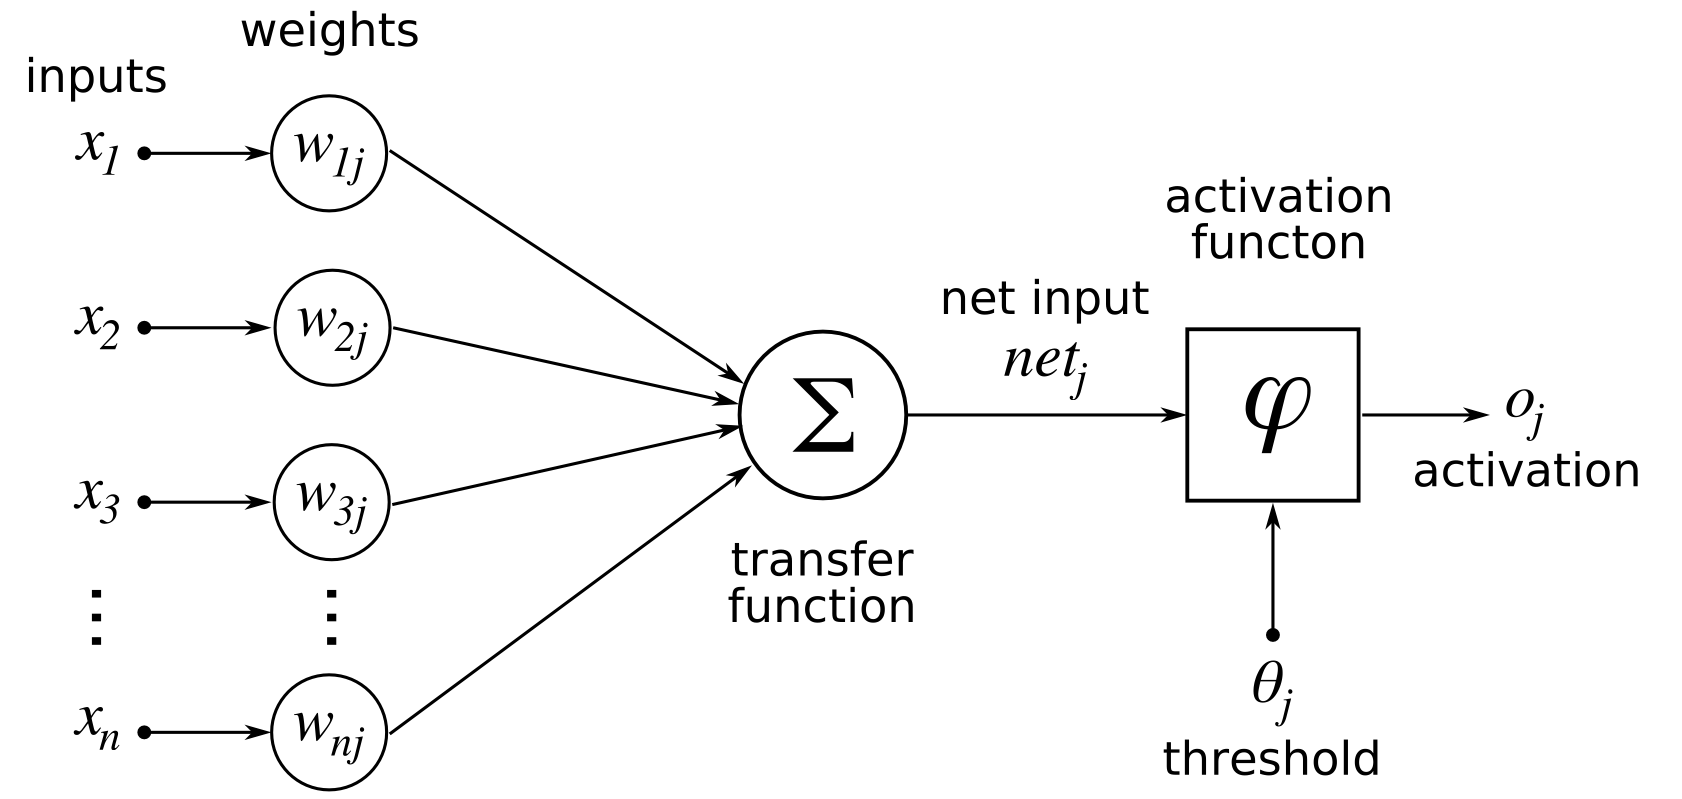
\includegraphics[scale=0.15]{./figure/nn_neuron.png}

\caption[A parallelism between a human-brain neuron and a neuron in a Brain Inspired Network]{A parallelism between a human-brain neuron and a neuron in a Brain Inspired Network\protect\footnotemark}
\label{fig:neuron}
\end{figure}

In the human brain, the basic computational unit is the neuron.\\ Neurons receive input signal from dendrites and produce output signal along the axon which interacts with other neurons via synaptic weights.\\ The synaptic weights are obtained after a learning process, which can strengthen them or not.
\footnotetext{Figures under CC license}
\subsubsection{Neural Networks}

Neural Networks (or Artificial Neural Networks) are graphs in which every node is interconnected to others using edges, which have a weight properly tuned during the training process.\\\\
As mentioned before, each and every node of the neural networks is called artificial neurons (a loosely model of its biological counterpart) and the connections (synapses in biological brain) can transmit information from a neuron to another. In Figure \ref{fig:neuron} the neurons receive signals, which is processed internally, and then they propagate it to the other connected neurons.\\\\
The information exchanged between a neuron and another is a real number, a result of a non-linear function of the sum of all its input.

In the Figure \ref{fig:nn} an implementation of a Neural Network can be appreciated.
\begin{figure}[H]
\centering
\captionsetup{justification=centering}
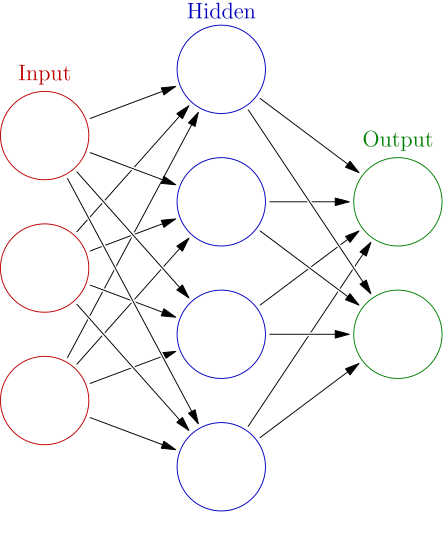
\includegraphics[scale=0.55]{./figure/neural_network.png}
\caption{Example of a Neural Network}
\label{fig:nn}
\end{figure}
As it can be seen in Figure \ref{fig:nn}, it is always divided in layers in which only the output and input layers are visible from the external world, as consequence the internal layers are called hidden layers. When an input vector is applied, it will propagate from the left side of the network to its right side through the layers and the neurons which compose each layer. It is worth to mention that layers may perform different kind of computation on their inputs. Moreover, the deep neural networks are named after the huge amount of hidden layers.\\\\

In the early stages of ANNs the goal was to solve problems as the human brain would do. However, over time, the aim moved to perform specific tasks, leading to a different architecture of the biological brain and brain-inspired networks (Spiking Neural Networks).\\\\
Depending on how the edges are connected and the topology, a Neural Network can be classified in several sub-types:
\begin{itemize}
\item Feed forward, the data move only from input layer to output layer without cycles in the graph.
\item Regulatory feedback, it provides feedback connections back to the same inputs that active them, reducing requirements during learning. It also allows learning and updating much easier.
\item Recurrent neural network, it propagates data backward and forward, from later processing stages to earlier stages.
\item Modular, several small networks cooperate or compete to solve problems.
\item Physical, it is based on electrically adjustable resistance material to simulate artificial synapses.
\end{itemize}

\subsubsection{Spiking Neural Networks}
Spiking neural networks (SNNs) are artificial neural networks that more closely mimic natural neural networks \cite{article:1}. \\\\In addition to neuronal and synaptic state, in their operational model, SNNs adds the concept of time. The idea is that neurons in the SNN do not activate at each propagation cycle but rather activate only when specific value is reached.\\\\
The current activation level is modeled as a differential equation and it is normally considered as neuron's state.

In principle, SNNs can be applied to the same application of Artificial Neural Networks. Moreover, SNNs can model brain of biological organisms without prior knowledge of the environment. Thus, SNNs have been useful in neuroscience for evaluating the reliability of the hypothesis on biological neural circuits but not in engineering.\\\\
SSNs are still lagging ANNs in terms of accuracy, but the gap is decreasing and has vanished on some task\cite{article:2}. However, computer architectures based on SNN have a huge energy footprint compare to other types of architecture \cite{paper:44}.
\newpage
\section{Machine Learning Quantization}
The reduction of computation demand, the increase of power efficiency and the memory footprint of machine learning algorithms can be achieved through the quantization.\\\\

Quantization is basically a set of techniques which convert, and map, input values from a large set to output values in a smaller set.\\\\The idea of Quantization is not recent, it has been introduced since the birth of digital electronics. Imagine taking a picture with the phone's camera, the real world is analog and the camera is capturing the analog world and converting it into a digital format. Nevertheless, the high quality of nowadays pictures, quantization is not lossless.\\\\
A trivial quantization example for Neural Network model is given in the below figure, where a set of potentially infinite value(floating-point) are mapped to finite values (integer).
\begin{figure}[H]
\centering
\captionsetup{justification=centering}
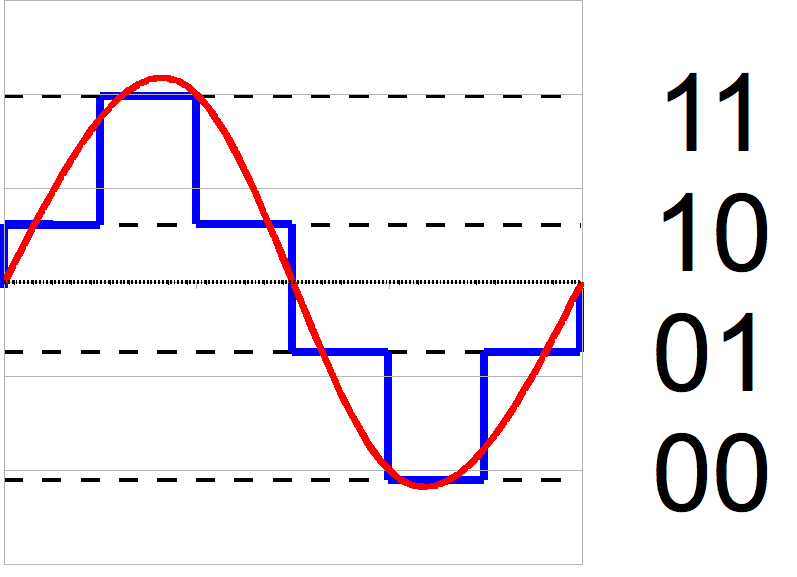
\includegraphics[scale=0.55]{./figure/quant.png}
\caption{Approximation of floating-point values to integer values}
\label{fig:quant}
\end{figure}
It has been proved that even if the model has been quantized, for example from fp32 to integer32, its accuracy is still good and the accuracy drop between the two data representation is negligible \cite{paper:8}.\\
Several quantization techniques can be applied, together or separated, to already trained ML models (post-training quantization):
\begin{itemize}
\item Linear quantization: data are directly scaled by taking their maximum value and normalizing them to falling in the desired range.
\item Outlier channel splitting \cite{paper:46} : linear quantization is sensitive by large inputs. The idea of OCS is to reduce the value of outliers (for both weights and activations) duplicating the node with halving the output or the weight. This transformation leaves the node functionality equivalent while at the same time it narrows the weight/activation distribution allowing a better linear quantization.
\item Analytical Clipping for Integer Quantization \cite{paper:47}: it represents the state-of-the-art for the post-training quantization techniques. It basically consists into apply a clipping function in a given range in order to reduce the quantization noise.
\end{itemize}

On the other hand, a quantization-aware training can also be done \cite{paper:45}.\\
Quantization has lead to a relief of hardware computation, as it is very well-known floating-point operation are much more expensive than integer operation from a lot of perspectives, and as consequence a reduction into the power consumption of the algorithm. It is also important to mention that the data traffic between the memory and the hardware is reduced due to the compaction of data.\\\\

Nowadays, edge devices take advantage of lower precision and quantized operations, including GPUs. Thus, quantization of machine learning algorithms is a defacto standard for edge inference.

\section{Applications}
In principle the AI can be applied to any intellectual tasks \cite{book:1}. Focusing on machine learning applications, they can spread through a variety of different domains:
\begin{itemize}
\item Healthcare, mainly used for classification purposes.
\item Automotive, used in self-driving cars.
\item Finance and economics, to detect charges or claims outside the norm, flagging these for human investigation. In banks system for organizing operations, maintains book-keeping, investing in stocks and managing properties.
\item Cybersecurity, automatically sort the data in networks into high risk and low-risk information.
\item Government, for paired with facial recognition systems may be used for mass surveillance.
\item Video games, it is routinely used to generate dynamic purposeful behavior in non-player characters.
\item Military, enhancing Communications, Sensors, Integration and Interoperability.
\item Hospitality, to reduce staff load and increase efficiency.
\item Advertising, it is used to predict the behavior of customers from their digital footprint in order to target them with personalized promotions.
\item Art, it has inspired numerous creative applications including its usage to produce visual art.
\end{itemize}
However, all the Machine Learning applications are characterized by the need of a huge amount of data set for the training process.
% CREATED BY DAVID FRISK, 2016
\chapter{System Development}

The designed accelerator has a Dataflow architecture, with emphasis on weight data reuse, and it is able to execute a tensor convolution. The basic idea is a computation matrix composed in every entry of processing elements which are able to perform operation between the incoming data and the weights, which have been already loaded for exploiting a data reuse approach.\\
The custom hardware accelerator is not useful as it is. It has to be integrated into a ML-Framework, TensorFlow, which allows to integrate a custom hardware accelerator minimizing the efforts to change the model code and its definitions.

The workflow of the Hardware-Software development is illustrated in the Figure \ref{fig:workflow}.
\begin{figure}[!htbp]
\centering
\captionsetup{justification=centering}
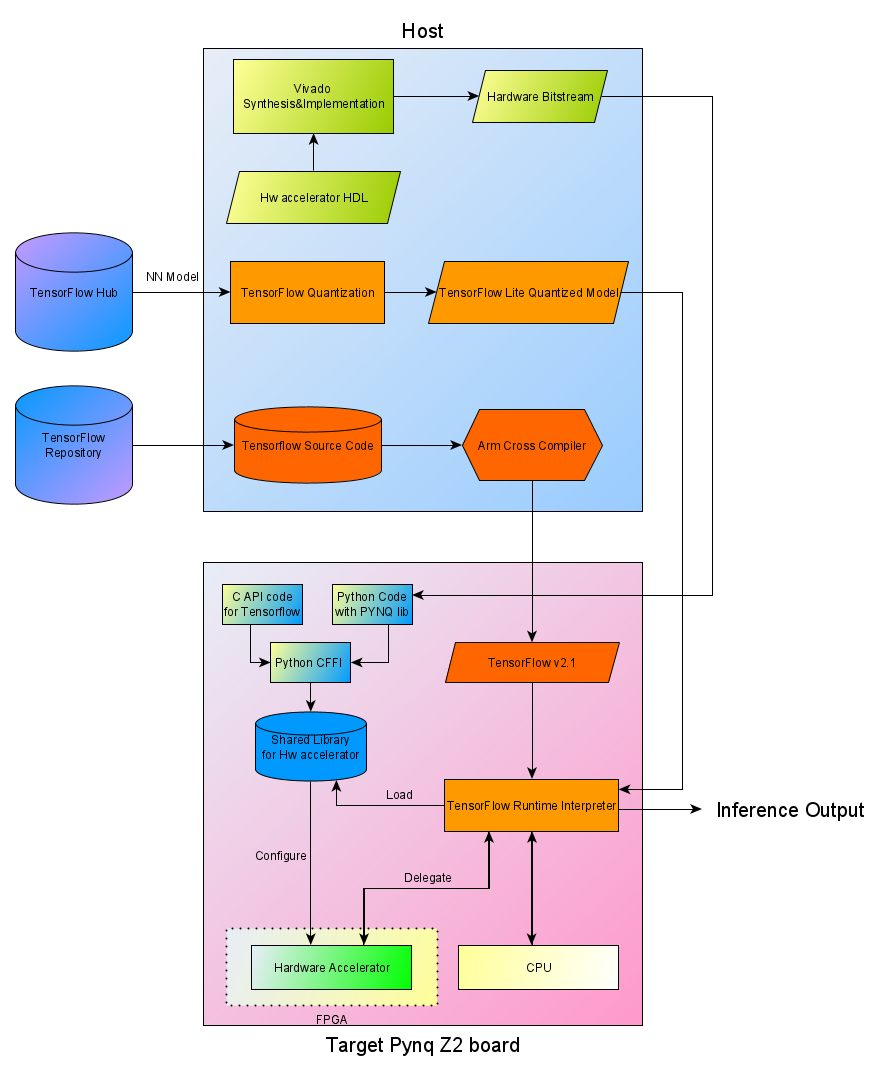
\includegraphics[scale=0.5]{./figure/workflow.png}
\caption{Development workflow}
\label{fig:workflow}
\end{figure}

\section{Software}

The focus of the work is the inference process, pre-trained models are needed and TensorFlow Hub comes in handy for this purpose. It provides already pre-trained Machine Learning models for different domains. Moreover, TensorFlow has the feature of quantizing a post-trained model for different arithmetic precision. In the Fig. \ref{fig:workflow} it can be seen that the quantization process has been done offline.\\
TensorFlow demands as library for the accelerator a C Python-API compatible shared library. In addition, the code for using the accelerator was already written using the PYNQ environment in Python. Therefore, for allowing code reuse and decreasing the development time the Python code has been embedded in the C code (from a TensorFlow example of the delegate library), adding callbacks to Python code.
\section{DTPU, the hardware accelerator}
The hardware accelerator, named \textit{Cogitantium\footnote{Thoughtful}, The Dumb Tensor Processing Unit}, is in charge of carrying out the tensor convolution of the neural network model, exploiting a data-flow architecture on the input data and a data reuse for the weight data.

The work is not focused on developing embedded memories and AXI interfaces, therefore a Xilinx's IP core, which includes all those necessary subcomponents, has been used.
The latter has allowed to completely focus the work on the DTPU core, which has become:
\begin{figure}[H]
\centering
\captionsetup{justification=centering}
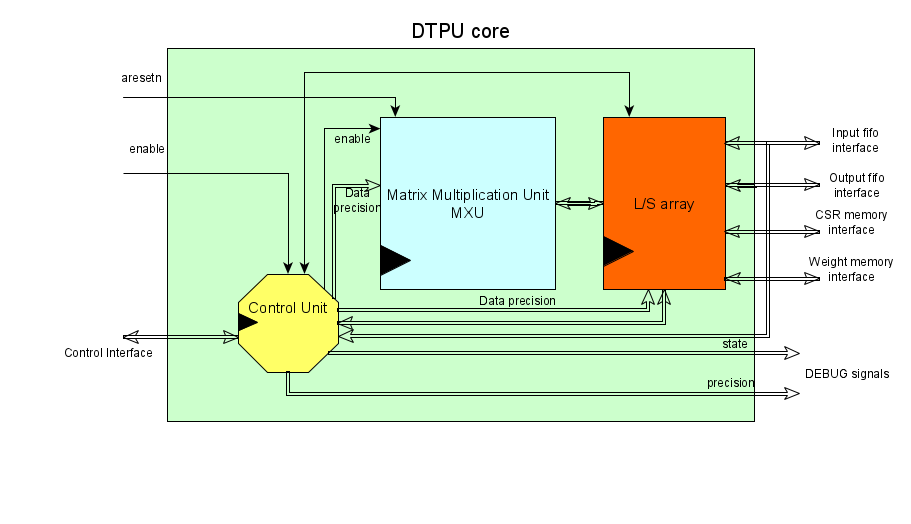
\includegraphics[scale=0.45,angle=0]{./figure/dtpu_core.png}
\caption{RTL view of DTPU core}
\label{fig:dtpucore}
\end{figure}
Where the sub-units:
\begin{itemize}
\item L/S array provides the data for the Matrix Multiplication Unit, especially the weight data are reused across several executions and therefore loaded once. It also provides the correct data to the correct computation units depending on the precision.
\item Control Unit is in charge of handling handshake signals for transferring the ownership of the data (data transferred by the DMA from the Main Memory), load the weights and activation in the respectively units and save the results to the output FIFO. Since it is a Data flow architecture, there is no control flow of the data in the core and this has allowed to keep the Control Unit as simple as possible.
\item Matrix Multiplication Unit (Mxu) is the computation unit of the hardware accelerator, the brawn of the accelerator, a symmetric matrix of MACs with variable precision, where every MAC unit has its own weight value. It executes the tensor convolution for different arithmetic precision.
\end{itemize}
% CREATED BY DAVID FRISK, 2016
\chapter{Results}
Every domain and application could have different evaluation metrics. In the following the overall metrics are evaluated.
\begin{itemize}
\item Utilization factor, for integer 8 and 16 the trend is similar. It is a 1 to 1 mapping between the PEs and the DSPs. As soon as the DSP are used the utilization of LUT and FF is linear in the sizes of Matrix Multiplication unit, while the DSP utilization is quadratic. At a full utilization of DSP entities the PEs start to be implemented in logic there is a sudden rise in the LUT utilization. Increasing the clock frequency, the FPGA's utilization is reduced since with an increase of the Matrix Multiplication Unit sizes the design is not able anymore to meet the timing requirements.
\item Energy and Power Consumption, the power consumption of the processing system and the static power consumption have a less impact on the total power consumption with an increase of the Matrix Multiplication Unit and the frequency. On the other hand, the dynamic power consumption, as expected, grows with a growing Matrix Multiplication Unit and the design frequency.
\item Throughput, it results to be equal to the number of rows into the Matrix Multiplication Unit. Enough data needs to be provided to the accelerator in order to have all the Processing Elements working with useful data, if not, the throughput goes down.
\item Latency, the execution of the models is done with different clock frequencies and data type, and as consequence a different overall latency (and power consumption). The reason about the increase in the latency, since the main goal was to reduce the latency, is that introducing the accelerator and its library comes with several overheads, mainly due to runtime transformations of matrices in a suitable format for the accelerator.
\item Accuracy, it is measured for different data width and model with reference to the actual value (inference without the accelerator). In general, models have a wrong prediction. One of the reason may reside in the input data feed to the model, they are totally random. Another improvement should be to accumulate on the different bit width precision, for example compute multiplication on 8 bits integer and accumulate values on 16-bit integer. Moreover, as in every software product, bugs have not been detected but this does not mean that the written software is bug-free.
\end{itemize}
% CREATED BY DAVID FRISK, 2016
\chapter{Conclusion}

\section{Discussion}A big portion of inference process for Neural Networks involves massive multiply and add computation, basic operation of tensor convolutions, and across several execution data, especially weight tensors, are reused.\\As consequence, for speeding-up and reduce the power consumption (especially in mobile devices) of ML models a hardware accelerator has been developed.
It is also designed for accommodating different data type computation request from Neural Network models, ranging from integer8/16/32/64 to floating-point 32 and brain floating-point 16.
It is possible to build a custom hardware accelerator for a specific ML operation and then integrate it into a framework without changing the model nor the framework.
The bottom up approach and the delegate class available in Tensorflow has allowed to fully tailor a new class of hardware accelerators which can accommodate different needs (i.e. depending on which part of the model has to be accelerated). As it has been organized, changing the core software in the Python code and the core in the hardware, it can be also used for addressing different model's operations.

\section{Future Works}
For every human artifacts, there is always work to do. In addition, for Computer Engineering artifacts there is also an important step which is the software (and in this case also of the hardware) optimization.
In particular:
\begin{itemize}
\item Software Optimization and migration to a full C code implementation for further reducing the latency.
\item A deep software/hardware testing for finding additional bugs.
\item Power estimation using the simulation’s switching activity in order to obtain a very precise and reliable power consumption.
\item Comparison of model execution on different state-of-the-art platforms.
\end{itemize}

Following the previous recommendation, the work may arrive to a competitive level such as the one of the GPUs or other hardware platforms.
\end{document}